\chapter[Project schedule and resource allocation]{Project schedule\newline{}and resource allocation}\label{chap:allocation}

%2. Identify the tasks for your project and their schedule. Do so retrospectively, assuming that the project has started in October 2015 as it really happened.

%3. Allocate the resources (all members of your group) to the various tasks. In defining the allocation, take into account your actual availability for the project.

%ALSO, considerazioni sui valori di tempo (e, t).

Following the estimations about cost, effort and time to develop myTaxiService, it is appropriate to define the scheduling of the development and implementation of the system. 

Le us start with the phases we already have gone though. For each, denoted by the abbreviation of the relating final document, we provide the total number of hours we dedicated to it (\textsc{H}), the actual available time (\textsc{AT}) and an estimate (\textsc{ET}) of how much time we would have needed, in case of full-time commitment (2~people, working 8~hours/day each)\footnote{The elements in this column are computed as follows:{\setlength{\mathindent}{.5cm} \begin{equation*}
	\text{\textsc{ET}} = \left\lceil \frac{\text{\textsc{H}}}{2 \text{ people}} * \frac{1}{8 \text{ hours}} \right\rceil
\end{equation*}}}. 

\begin{table}\centering\begin{tabular}{ >{\ttfamily}c c c c }

\toprule
\normalfont\textsc{Phase} & \normalfont\textsc{H} & \normalfont\textsc{AT} & \normalfont\textsc{ET} \\
\toprule

RASD & 		61 &	3 weeks & 	$\simeq$ 4 days \\\midrule
DD &		68 &	4 weeks & 	$\simeq$ 5 days \\\midrule
ITPD &		10 &	2 weeks &	$\simeq$ 1 day  \\\midrule
PPD &		XX &	2 weeks & 	$\simeq$ X days \\

\bottomrule
	
\end{tabular}
\vspace{\baselineskip}
\end{table}
% TODO Correggi PPD!!!!!


Notice that it is nearly impossible for us to define a role for the two of us in the team, because we always worked together on the whole documents. 

Obviously, the time in \textsc{ET} is an underestimation. If we had the chance to dedicate our full time to the project, many more aspects would have been analysed (e.g., on the physical architecture of the system, the issue of code reusing, the system and performance testing), which would have required more time. 

Now we want to relate these results with the time to develop $ \mathbf{t} = 40 \text{ weeks} $, computed in \cref{eqn:timeVAL}. Following COCOMO definition, this parameter considers the span of time between the beginning of the design phase and the end of the integration testing. In particular, we can identify the following phases which naturally occur in the considered span of time: \begin{enumerate}
	
	\item Product planning and detailed design phase (\texttt{DD}, \texttt{ITPD}, and \texttt{PPD});
	
	\item Code and unit test phase. 
	
	\item Integration and test phase. 
	
\end{enumerate}

As one can notice, the first phase is now completed with the delivery of this document. This means that we now have the following number of weeks to develop, integrate and test the system:\begin{equation}
%
\mathbf{t} - 2 * \left\lceil \frac{ \text{ \textsc{EM}(\texttt{DD})} +  
									\text{\textsc{EM}(\texttt{ITPD})} +
									\text{\textsc{EM}(\texttt{PPD}) }
								   }{7} \right\rceil = XX
%	
\end{equation}

With the doubled ceiling operation we are computing the ``corrected'' number of weeks (considering the issue of the underestimation, mentioned above) needed for the planning and design phase.

As of the development, we identify some critical components, which need to be developed as early as possible. In particular we notice that \texttt{Area\-Man\-age\-ment}, \texttt{Re\-quest\-Man\-age\-ment}, and \texttt{Re\-quest\-Cre\-ation} are fundamental to allow the development the other components of the system, so they have to be developed first (and unit tested, of course). 

On the other hand, \texttt{Res\-er\-va\-tion\-Cre\-ation} and \texttt{Res\-er\-va\-tion\-Man\-age\-ment} are far less critical, as the first release of the software system may not even include this functionality. 

However, we find it pointless to prescribe the allocation of coding tasks to each developer, so we are not going to. We only suggest to dedicate about one third of the time to the integration testing phase, as we believe it to be crucial for the quality of the system.








\begin{comment}
	




%TODO Correggi: RASD esterno.
\begin{figure*}%
	\includestandalone[mode=tex, width=\textwidth]{img/gantt/gantt}
	\caption{myTaxiService Gantt chart.}\label{fig:gantt1}
\end{figure*}


\begin{figure*}
%	Textwidth: \the\textwidth
	\newlength{\imagewidth}%
	\settowidth\imagewidth{\input{img/ganttDEV/ganttDEV}}%
	\includestandalone[mode=tex, width=.81\imagewidth]{img/ganttDEV/ganttDEV}
\end{figure*}



The following phases are identified:\begin{description}
	\item [\normalfont\texttt{RASD}] requirements analysis and specification; the resulting document, which required three weeks, was delivered on \printdate{2015-11-6}.
	\item [\normalfont\texttt{DD}] designing; the resulting document, which required four weeks, was delivered on \printdate{2015-12-4}.
	\item [\normalfont\texttt{ITPD}] integration testing plan; the resulting document, which required three weeks, was delivered on \printdate{2016-1-21} (notice that there is a temporal hiatus between the previous phase and this one).
	\item [\normalfont\texttt{PPD}] project planning; the resulting document, which required three weeks, is this one, and is going to be delivered on \printdate{2016-2-2}.
	\item [\normalfont\texttt{Dev}] development and unit testing; this phase will require about 21 weeks; in a few lines, we are going to detail this phase.
	\item [\normalfont\texttt{Int}] integration and testing; eight weeks will be dedicated to this phase.
\end{description}



As of the development phase, we are now presenting again in \cref{fig:intsequence} the sequence of integration scheme (already introduced in the \emph{Integration testing plan document}), because it gives a reasonable view on the critical components which need to be developed first.


\begin{figure*}
	\centering
	\includestandalone[mode=tex, width=\textwidth]{img/sequence/sequence_o}  
	\caption{Sequence of development and integration.}
	\label{fig:intsequence}
\end{figure*}



As of the development phase, we are presenting again in \cref{fig:component} the well known component diagram of myTaxiService system. 


\begin{figure*}
	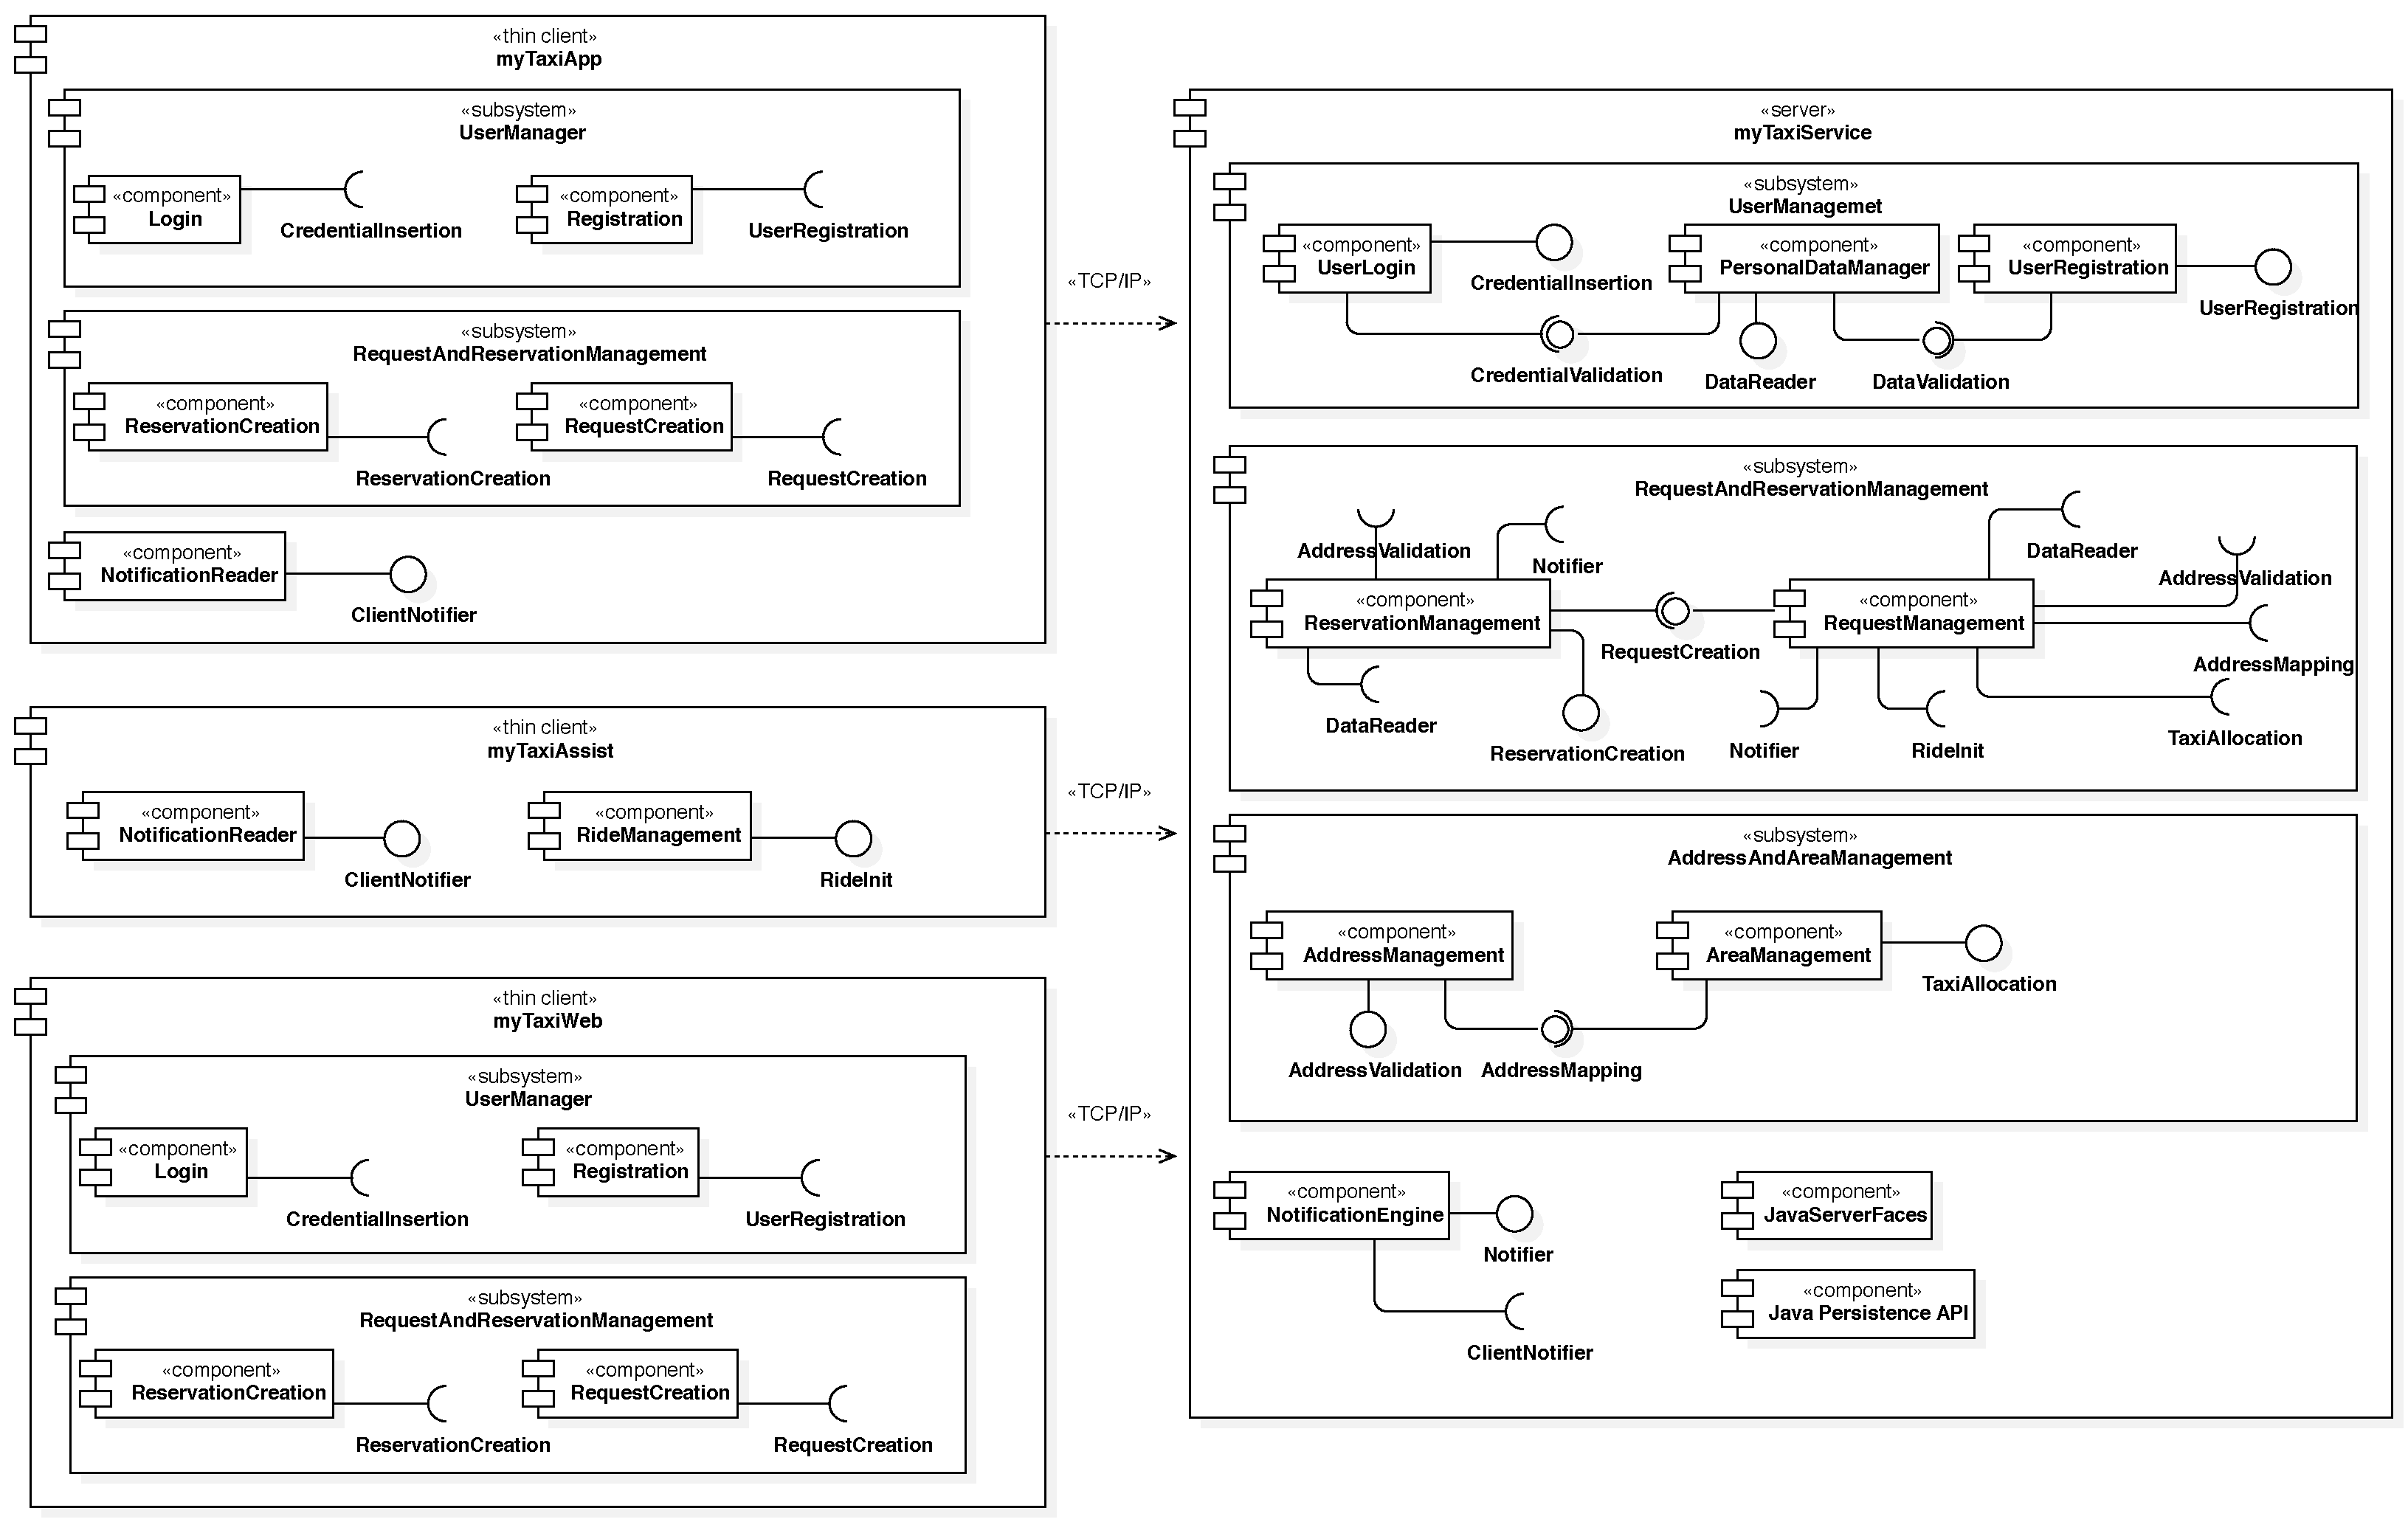
\includegraphics[width=\textwidth]{img/ComponentView__ComponentDiagram_1}
	\caption{Component diagram.}
	\label{fig:component}
\end{figure*}














\end{comment}












